\chapter{Mathematical Modelling of First-Order Equations}

\chapter*{Lecture 9}
\begin{recall}{}{}
\begin{itemize}
\item Finalized chapter 2 
\end{itemize}
\end{recall}




\section{Mathematical Modelling}

Approach towards mathematical modelling:
\begin{enumerate}
\item Problem statement
\begin{itemize}
\item Pictoral representation of the system
\item Identify important physical parameters
\item Determine the variable you want to find
\end{itemize}

\item Formulate the mathematical model
\begin{itemize}
\item Use physical laws to express the problem mathematically
\item Identify initial/boundary conditions
\end{itemize}
\item Solve the problem
\begin{itemize}
\item Find the functional form of the parameters of interest
\item Solve for any particular cases
\item Check to see if the form of the solution makes sense
\end{itemize}
\item Analysis
\begin{itemize}
\item Answer the posed problem
\end{itemize}
\end{enumerate}

\begin{center}
\noindent\rule{4cm}{0.4pt}
\end{center}


%=================
\begin{exmp}{Water level in tank:}\\
\begin{minipage}{0.65\textwidth}
We want to know the level of the water in a 50~cm-diameter tank with a 5mm-diameter hole in the bottom. The water exits at a rate of $\dot{V}=A_e \sqrt{2gy}$, where  $y$ is the height of water. The initial water level is 1 m. Knowing $g=9.8$ m/s$^2$, find the height of water in the tank as a function of time.\\
\end{minipage}
\hspace{0.05\textwidth}
\begin{minipage}{0.27\textwidth}
\centering
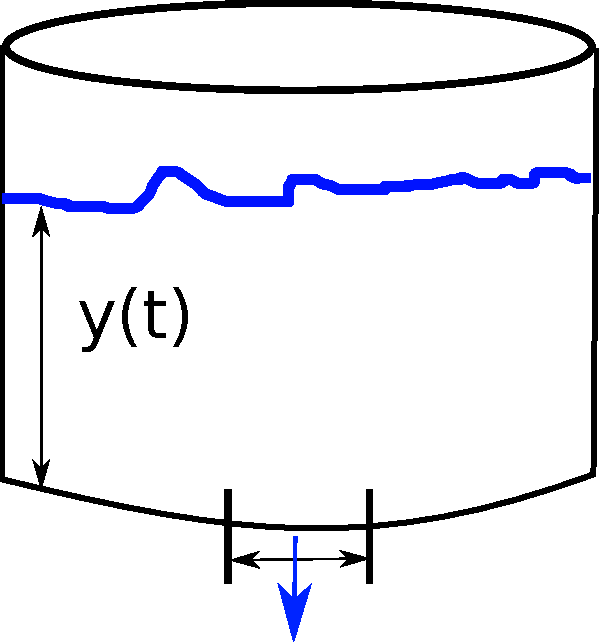
\includegraphics[width=\textwidth]{figs/tankProblem.pdf} 
\end{minipage}

 \textbf{Solution:} \\
\begin{enumerate}
\item \textbf{Problem statement}
\begin{itemize}
\item Pictoral representation (check)
\item Variables $y(t)$, $t$
\item Parameters: Diameter of tank: $D_t=50$ cm \\
  Diameter of exit hole: $D_t=5$ mm \\
  $g=9.8 m/s^2$
\end{itemize}
\item \textbf{Formulate mathematical model}
\begin{itemize}
\item Physical conservation law: conservation of mass or volume
\item Mathematical expression:
\begin{equation*}
\frac{d m(t)}{dt}= \dot{m}_{in}-\dot{m}_{out}\qquad or \qquad\frac{d V(t)}{dt}= \dot{V}_{in}-\dot{V}_{out}
\end{equation*}
\item Translate physical law to an ODE for the dependent variable $y$:
\begin{equation*}
V=\frac{\pi}{4}D^2_t y \qquad or \qquad \frac{d V(t)}{dt}= \frac{\pi}{4}D^2_t \frac{d y(t)}{dt} 
\end{equation*}
We must also account for the $\dot{V}_{in}$ and $\dot{V}_{out}$ terms:
\begin{equation*}
\dot{V}_{in}=0 \qquad \dot{V}_{out}=?
\end{equation*}
How do we determine the exit volumetric flow rate leaving the tank?
\begin{itemize}
\item Volume flow rate $[m^3/s]$ represents a velocity times and area. Therefore, we want to find the velocity at the exit, $U$.
\item Let's consider a conservation of energy equation (writen as the Bernoulli equation) for hydrostatics between point A (at $y(t)$) and point B (at exit):
\begin{equation*}
\frac{p_{A}}{\rho_A}+gy_A+\frac{U^2_A}{2}=
\frac{p_{B}}{\rho_B}+gy_B+\frac{U^2_B}{2}
\end{equation*}
(note $\rho$ corresponds to the density of the fluid) Through simplification we find:
\begin{equation*}
gy_A=\frac{U^2_B}{2}
\end{equation*}
or $U_B=\sqrt{2gy}$
\end{itemize}
Therefore, our volumetric flow rate leaving the tank is: $\dot{V}_{out}=A_e\sqrt{2gy}$ or $\dot{V}_{out}=\frac{\pi}{4}D^2_e\sqrt{2gy}$
\item Our ODE becomes:
\begin{equation*}
\frac{\pi}{4}D^2_t \frac{d y(t)}{dt} =-\frac{\pi}{4}D^2_e\sqrt{2gy}
\end{equation*}
\item Standard form:
\begin{equation*}
 \frac{d y(t)}{dt} =-\frac{D^2_e}{D^2_t}\sqrt{2gy}
\end{equation*}
\item Initial conditions: $y(0)=1$
\end{itemize}
\item \textbf{Solve the ODE:} The equation can be solved by separation and direct integration:
\begin{equation*}
\int \frac{1}{\sqrt{y}}dy=-\frac{D^2_e}{D^2_t}\sqrt{2g}\int\, dt +c
\end{equation*}
yields:
\begin{equation*}
2\sqrt{y}=-\frac{D^2_e}{D^2_t}\sqrt{2g} \, t +c
\end{equation*}
or:
\begin{equation*}
y=\left(-\frac{D^2_e}{2D^2_t}\sqrt{2g} \, t +c\right)^2
\end{equation*}
This is the \textbf{general solution}. We apply the IC to this equation:
\begin{equation*}
1=\left(-\frac{D^2_e}{2D^2_t}\sqrt{2g} \, (0) +c\right)^2
\end{equation*}
therefore $c=\pm 1$. We choose $+1$, why? 

The final \textbf{particular solution} is:
\begin{equation*}
\boxed{y=\left(1-\frac{D^2_e}{2D^2_t}\sqrt{2g} \, t \right)^2=\left(1-0.000221t\right)^2}
\end{equation*}
\item \textbf{Further studies}
Example: At what time will the tank be completely empty? In other words, find $t$ for $y=0$. Approx 75 min.

\end{enumerate}
\end{exmp}


\begin{center}
\noindent\rule{4cm}{0.4pt}
\end{center}
\updateinfo[September 25, 2018]
